% Circuit: Nested-LCU block encoding U_{B_a} --- SELECT controls drawn as
%          half-filled disks (bottom-right black, upper-left white) to signal
%          that the control is uniform over the bundled time register.
% Generated for: QuantumFurnace.jl PhD thesis (Chapter 5, Methods; Alg. 1a / alg:coh).
% Usage: % Circuit: Nested-LCU block encoding U_{B_a} --- SELECT controls drawn as
%          half-filled disks (bottom-right black, upper-left white) to signal
%          that the control is uniform over the bundled time register.
% Generated for: QuantumFurnace.jl PhD thesis (Chapter 5, Methods; Alg. 1a / alg:coh).
% Usage: % Circuit: Nested-LCU block encoding U_{B_a} --- SELECT controls drawn as
%          half-filled disks (bottom-right black, upper-left white) to signal
%          that the control is uniform over the bundled time register.
% Generated for: QuantumFurnace.jl PhD thesis (Chapter 5, Methods; Alg. 1a / alg:coh).
% Usage: % Circuit: Nested-LCU block encoding U_{B_a} --- SELECT controls drawn as
%          half-filled disks (bottom-right black, upper-left white) to signal
%          that the control is uniform over the bundled time register.
% Generated for: QuantumFurnace.jl PhD thesis (Chapter 5, Methods; Alg. 1a / alg:coh).
% Usage: \input{circuits/block-encoding-ba-halfctrl.tex} in the main thesis,
%        or compile standalone.
%
% Differences from block-encoding-ba.tex:
%   (1) \ctrl{n}  -->  \ctrl[style=halfctrl]{n}  on every SELECT control
%       (cells 4, 12 on T_-; cells 6, 8, 10 on T_+).
%   (2) Signed/complex LCU fix, matching Chen et al. Fig. 4:
%         - left-side PREP on each register prepares the *signed* state
%               |b'_->   = sum_t   [b_-(t)/sqrt(|b_-(t)|)] / sqrt(||b_-||_1) |t>
%               |b'_+>   = sum_t'  [b_+(t')/sqrt(|b_+(t')|)] / sqrt(||b_+||_1) |t'>
%           denoted PREP'_- and PREP'_+ (primed).
%         - right-side PREP on each register prepares the *magnitude* state
%               |b_->    = sum_t   sqrt(|b_-(t)| / ||b_-||_1) |t>
%               |b_+>    = sum_t'  sqrt(|b_+(t')| / ||b_+||_1) |t'>
%           denoted PREP_- and PREP_+ (unprimed), and enters the circuit as
%           its adjoint PREP^dag on the right end.
%       With these two distinct preps, the left*right amplitude product on
%       each register is
%               [sgn/phase(b_-) sqrt(|b_-|)] * sqrt(|b_-|)  =  b_-
%       recovering the correctly signed/phased linear combination.
%       A symmetric PREP/PREP^dag on both ends would instead block-encode
%       |b_-(t)| (losing the sign), which is the wrong operator.
%
\documentclass{article}
\usepackage[margin=1cm]{geometry}
\usepackage{tikz}
\usetikzlibrary{quantikz2}
\usepackage{amsmath,amssymb}
\usepackage{braket}

\newcommand{\ee}{\mathrm{e}}
\newcommand{\ii}{\mathrm{i}}

% Rounded corners on all gates globally
\tikzset{operator/.append style={rounded corners}}

% Half-filled control: disk split by a / diagonal,
% lower-right triangle black, upper-left triangle white.
% Denotes a SELECT-style control that is *uniform* over a bundled register,
% as opposed to a computational-basis control on a single wire.
\tikzset{
  halfctrl/.style={
    circle, draw=black, line width=0.4pt,
    fill=white, minimum size=6pt, inner sep=0pt,
    path picture={
      \fill[black]
        (path picture bounding box.south west) --
        (path picture bounding box.south east) --
        (path picture bounding box.north east) -- cycle;
      \draw[black, line width=0.3pt]
        (path picture bounding box.south west) --
        (path picture bounding box.north east);
    }
  }
}

\begin{document}
\pagestyle{empty}

\begin{figure}[ht]
  \centering
  \makebox[\textwidth][c]{%
  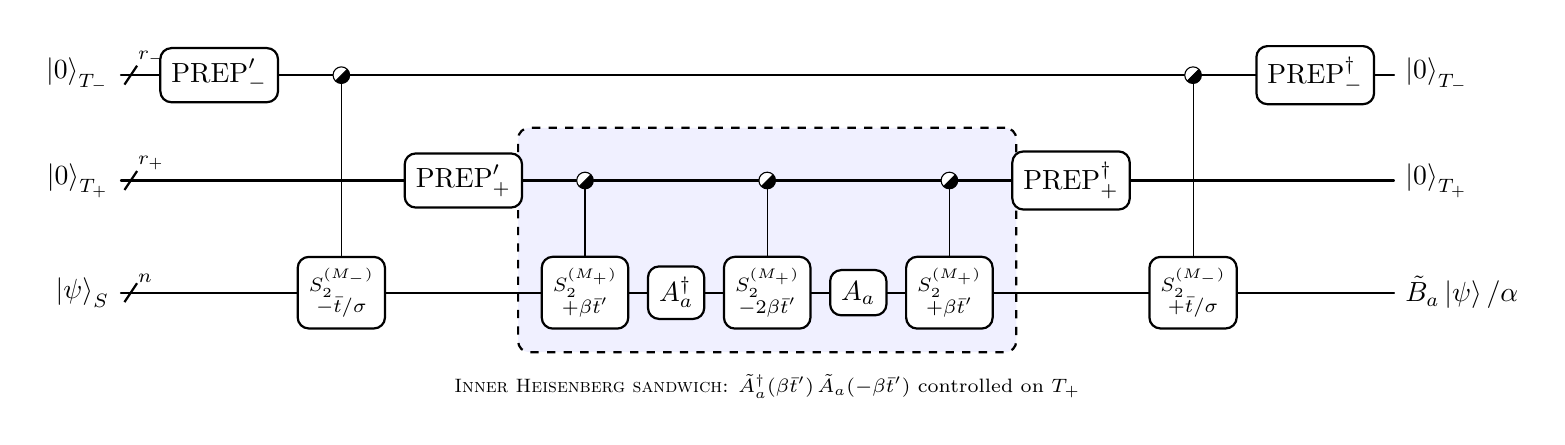
\begin{tikzpicture}
  \node[scale=1.0]{%
  \begin{quantikz}[row sep=0.6cm, column sep=0.25cm]
  %
  % Cell-by-cell layout (14 cells per row):
  %   1: \lstick                  (left label)
  %   2: wire decl                (\qwbundle{...})
  %   3: PREP'_-  (signed, outer)
  %   4: Ctrl-Trott outer^-       (S_2(-bar t / sigma) on S, ctrl on T_-)
  %   5: PREP'_+  (signed/phased, inner)
  %   6: Ctrl-Trott inner^+       (S_2(+beta bar t') on S, ctrl on T_+)
  %   7: A_a^dag on S             (inner Heisenberg sandwich, left)
  %   8: Ctrl-Trott inner^-2      (S_2(-2 beta bar t') on S, ctrl on T_+)
  %   9: A_a on S                 (inner Heisenberg sandwich, right)
  %  10: Ctrl-Trott inner^+       (S_2(+beta bar t') on S, ctrl on T_+)
  %  11: PREP_+^dag  (magnitude, inner UNPREP)
  %  12: Ctrl-Trott outer^+       (S_2(+bar t / sigma) on S, ctrl on T_-)
  %  13: PREP_-^dag  (magnitude, outer UNPREP)
  %  14: rstick
  %
  % ==================================================================
  % Row 1:  T_-  (outer time register; controls cells 4 and 12)
  % ==================================================================
    \lstick{$\ket{0}_{T_-}$}
      & \qwbundle{r_-}
      & \gate{\text{PREP}'_-}
      & \ctrl[style=halfctrl]{2}
      & \qw
      & \qw
      & \qw
      & \qw
      & \qw
      & \qw
      & \qw
      & \ctrl[style=halfctrl]{2}
      & \gate{\text{PREP}_-^\dagger}
      & \rstick{$\ket{0}_{T_-}$}\qw
      \\
  %
  % ==================================================================
  % Row 2:  T_+  (inner time register; controls cells 6, 8, 10;
  %              prepared in cell 5, uncomputed in cell 11)
  % ==================================================================
    \lstick{$\ket{0}_{T_+}$}
      & \qwbundle{r_+}
      & \qw
      & \qw
      & \gate{\text{PREP}'_+}
      & \ctrl[style=halfctrl]{1}
      \gategroup[2,steps=5,style={dashed,rounded corners,fill=blue!6,inner sep=5pt},
                 background,label style={label position=below,yshift=-0.35cm,anchor=north}]
        {\scriptsize \textsc{Inner Heisenberg sandwich}:
         $\tilde{A}_a^\dagger(\beta\bar t')\,\tilde{A}_a(-\beta\bar t')$
         controlled on $T_+$}
      & \qw
      & \ctrl[style=halfctrl]{1}
      & \qw
      & \ctrl[style=halfctrl]{1}
      & \gate{\text{PREP}_+^\dagger}
      & \qw
      & \qw
      & \rstick{$\ket{0}_{T_+}$}\qw
      \\
  %
  % ==================================================================
  % Row 3:  S  (system register; target of every controlled evolution
  %             and of the two jump applications A_a^dag, A_a)
  % ==================================================================
    \lstick{$\ket{\psi}_S$}
      & \qwbundle{n}
      & \qw
      & \gate{\substack{S_2^{(M_-)} \\[-1pt] \scriptstyle -\bar t/\sigma}}
      & \qw
      & \gate{\substack{S_2^{(M_+)} \\[-1pt] \scriptstyle +\beta\bar t'}}
      & \gate{A_a^\dagger}
      & \gate{\substack{S_2^{(M_+)} \\[-1pt] \scriptstyle -2\beta\bar t'}}
      & \gate{A_a}
      & \gate{\substack{S_2^{(M_+)} \\[-1pt] \scriptstyle +\beta\bar t'}}
      & \qw
      & \gate{\substack{S_2^{(M_-)} \\[-1pt] \scriptstyle +\bar t/\sigma}}
      & \qw
      & \rstick{$\tilde B_a\ket{\psi}/\alpha$}\qw
  \end{quantikz}%
  };
  \end{tikzpicture}%
  }
  \caption{Nested-LCU block encoding $U_{B_a}$ of the Trotterized coherent
  Metropolis term $\tilde{B}_a/\alpha$ with $\alpha=\lVert b_-\rVert_1\lVert b_+\rVert_1$
  (Alg.~\ref*{alg:coh}, \eqref{eq:B-block-encoding}), on outer/inner time
  registers $T_\mp$; projection on $\ket{0}_{T_-}\!\ket{0}_{T_+}$ is implicit.
  Half-filled controls denote uniform (SELECT) control over the bundled time
  registers. Following \cite[Fig.~4]{chen2023efficient},
  $\text{PREP}'_\pm$ prepares the signed/phased state
  $\sum_{\bar t}[b_\pm(\bar t)/\sqrt{|b_\pm(\bar t)|}]\ket{\bar t}/\sqrt{\lVert b_\pm\rVert_1}$
  and $\text{PREP}_\pm$ the magnitude state
  $\sum_{\bar t}\sqrt{|b_\pm(\bar t)|/\lVert b_\pm\rVert_1}\ket{\bar t}$,
  so that amplitudes multiply to the signed kernel $b_\pm(\bar t)$. Controlled
  evolutions are Trotterized with the second-order Strang splitting $S_2^{(M_\pm)}$.}
  \label{fig:block-encoding-ba-halfctrl}
\end{figure}

\end{document}
 in the main thesis,
%        or compile standalone.
%
% Differences from block-encoding-ba.tex:
%   (1) \ctrl{n}  -->  \ctrl[style=halfctrl]{n}  on every SELECT control
%       (cells 4, 12 on T_-; cells 6, 8, 10 on T_+).
%   (2) Signed/complex LCU fix, matching Chen et al. Fig. 4:
%         - left-side PREP on each register prepares the *signed* state
%               |b'_->   = sum_t   [b_-(t)/sqrt(|b_-(t)|)] / sqrt(||b_-||_1) |t>
%               |b'_+>   = sum_t'  [b_+(t')/sqrt(|b_+(t')|)] / sqrt(||b_+||_1) |t'>
%           denoted PREP'_- and PREP'_+ (primed).
%         - right-side PREP on each register prepares the *magnitude* state
%               |b_->    = sum_t   sqrt(|b_-(t)| / ||b_-||_1) |t>
%               |b_+>    = sum_t'  sqrt(|b_+(t')| / ||b_+||_1) |t'>
%           denoted PREP_- and PREP_+ (unprimed), and enters the circuit as
%           its adjoint PREP^dag on the right end.
%       With these two distinct preps, the left*right amplitude product on
%       each register is
%               [sgn/phase(b_-) sqrt(|b_-|)] * sqrt(|b_-|)  =  b_-
%       recovering the correctly signed/phased linear combination.
%       A symmetric PREP/PREP^dag on both ends would instead block-encode
%       |b_-(t)| (losing the sign), which is the wrong operator.
%
\documentclass{article}
\usepackage[margin=1cm]{geometry}
\usepackage{tikz}
\usetikzlibrary{quantikz2}
\usepackage{amsmath,amssymb}
\usepackage{braket}

\newcommand{\ee}{\mathrm{e}}
\newcommand{\ii}{\mathrm{i}}

% Rounded corners on all gates globally
\tikzset{operator/.append style={rounded corners}}

% Half-filled control: disk split by a / diagonal,
% lower-right triangle black, upper-left triangle white.
% Denotes a SELECT-style control that is *uniform* over a bundled register,
% as opposed to a computational-basis control on a single wire.
\tikzset{
  halfctrl/.style={
    circle, draw=black, line width=0.4pt,
    fill=white, minimum size=6pt, inner sep=0pt,
    path picture={
      \fill[black]
        (path picture bounding box.south west) --
        (path picture bounding box.south east) --
        (path picture bounding box.north east) -- cycle;
      \draw[black, line width=0.3pt]
        (path picture bounding box.south west) --
        (path picture bounding box.north east);
    }
  }
}

\begin{document}
\pagestyle{empty}

\begin{figure}[ht]
  \centering
  \makebox[\textwidth][c]{%
  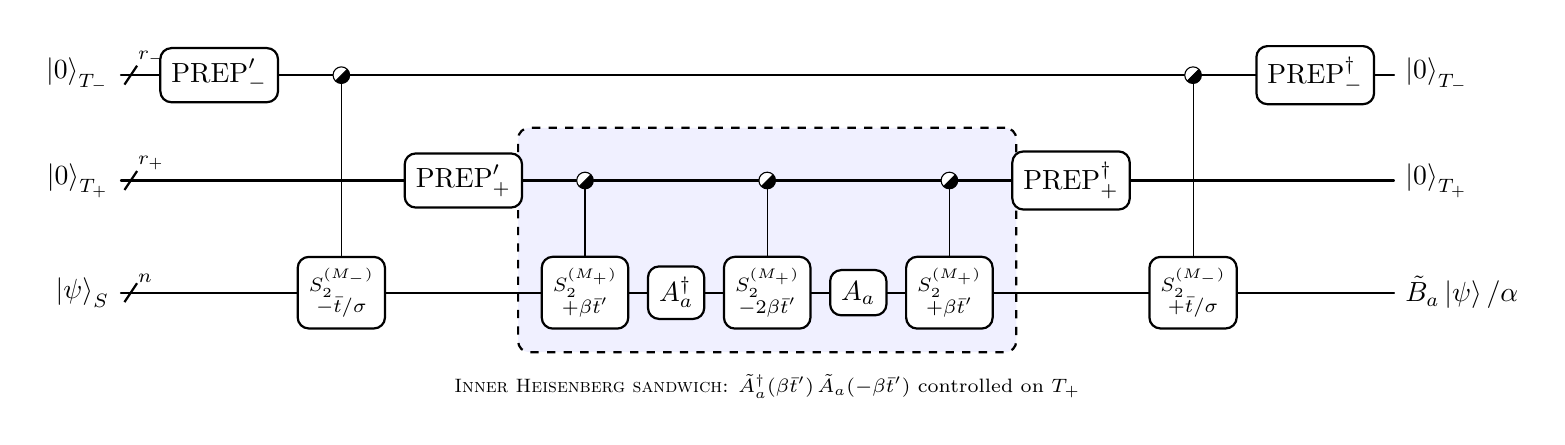
\begin{tikzpicture}
  \node[scale=1.0]{%
  \begin{quantikz}[row sep=0.6cm, column sep=0.25cm]
  %
  % Cell-by-cell layout (14 cells per row):
  %   1: \lstick                  (left label)
  %   2: wire decl                (\qwbundle{...})
  %   3: PREP'_-  (signed, outer)
  %   4: Ctrl-Trott outer^-       (S_2(-bar t / sigma) on S, ctrl on T_-)
  %   5: PREP'_+  (signed/phased, inner)
  %   6: Ctrl-Trott inner^+       (S_2(+beta bar t') on S, ctrl on T_+)
  %   7: A_a^dag on S             (inner Heisenberg sandwich, left)
  %   8: Ctrl-Trott inner^-2      (S_2(-2 beta bar t') on S, ctrl on T_+)
  %   9: A_a on S                 (inner Heisenberg sandwich, right)
  %  10: Ctrl-Trott inner^+       (S_2(+beta bar t') on S, ctrl on T_+)
  %  11: PREP_+^dag  (magnitude, inner UNPREP)
  %  12: Ctrl-Trott outer^+       (S_2(+bar t / sigma) on S, ctrl on T_-)
  %  13: PREP_-^dag  (magnitude, outer UNPREP)
  %  14: rstick
  %
  % ==================================================================
  % Row 1:  T_-  (outer time register; controls cells 4 and 12)
  % ==================================================================
    \lstick{$\ket{0}_{T_-}$}
      & \qwbundle{r_-}
      & \gate{\text{PREP}'_-}
      & \ctrl[style=halfctrl]{2}
      & \qw
      & \qw
      & \qw
      & \qw
      & \qw
      & \qw
      & \qw
      & \ctrl[style=halfctrl]{2}
      & \gate{\text{PREP}_-^\dagger}
      & \rstick{$\ket{0}_{T_-}$}\qw
      \\
  %
  % ==================================================================
  % Row 2:  T_+  (inner time register; controls cells 6, 8, 10;
  %              prepared in cell 5, uncomputed in cell 11)
  % ==================================================================
    \lstick{$\ket{0}_{T_+}$}
      & \qwbundle{r_+}
      & \qw
      & \qw
      & \gate{\text{PREP}'_+}
      & \ctrl[style=halfctrl]{1}
      \gategroup[2,steps=5,style={dashed,rounded corners,fill=blue!6,inner sep=5pt},
                 background,label style={label position=below,yshift=-0.35cm,anchor=north}]
        {\scriptsize \textsc{Inner Heisenberg sandwich}:
         $\tilde{A}_a^\dagger(\beta\bar t')\,\tilde{A}_a(-\beta\bar t')$
         controlled on $T_+$}
      & \qw
      & \ctrl[style=halfctrl]{1}
      & \qw
      & \ctrl[style=halfctrl]{1}
      & \gate{\text{PREP}_+^\dagger}
      & \qw
      & \qw
      & \rstick{$\ket{0}_{T_+}$}\qw
      \\
  %
  % ==================================================================
  % Row 3:  S  (system register; target of every controlled evolution
  %             and of the two jump applications A_a^dag, A_a)
  % ==================================================================
    \lstick{$\ket{\psi}_S$}
      & \qwbundle{n}
      & \qw
      & \gate{\substack{S_2^{(M_-)} \\[-1pt] \scriptstyle -\bar t/\sigma}}
      & \qw
      & \gate{\substack{S_2^{(M_+)} \\[-1pt] \scriptstyle +\beta\bar t'}}
      & \gate{A_a^\dagger}
      & \gate{\substack{S_2^{(M_+)} \\[-1pt] \scriptstyle -2\beta\bar t'}}
      & \gate{A_a}
      & \gate{\substack{S_2^{(M_+)} \\[-1pt] \scriptstyle +\beta\bar t'}}
      & \qw
      & \gate{\substack{S_2^{(M_-)} \\[-1pt] \scriptstyle +\bar t/\sigma}}
      & \qw
      & \rstick{$\tilde B_a\ket{\psi}/\alpha$}\qw
  \end{quantikz}%
  };
  \end{tikzpicture}%
  }
  \caption{Nested-LCU block encoding $U_{B_a}$ of the Trotterized coherent
  Metropolis term $\tilde{B}_a/\alpha$ with $\alpha=\lVert b_-\rVert_1\lVert b_+\rVert_1$
  (Alg.~\ref*{alg:coh}, \eqref{eq:B-block-encoding}), on outer/inner time
  registers $T_\mp$; projection on $\ket{0}_{T_-}\!\ket{0}_{T_+}$ is implicit.
  Half-filled controls denote uniform (SELECT) control over the bundled time
  registers. Following \cite[Fig.~4]{chen2023efficient},
  $\text{PREP}'_\pm$ prepares the signed/phased state
  $\sum_{\bar t}[b_\pm(\bar t)/\sqrt{|b_\pm(\bar t)|}]\ket{\bar t}/\sqrt{\lVert b_\pm\rVert_1}$
  and $\text{PREP}_\pm$ the magnitude state
  $\sum_{\bar t}\sqrt{|b_\pm(\bar t)|/\lVert b_\pm\rVert_1}\ket{\bar t}$,
  so that amplitudes multiply to the signed kernel $b_\pm(\bar t)$. Controlled
  evolutions are Trotterized with the second-order Strang splitting $S_2^{(M_\pm)}$.}
  \label{fig:block-encoding-ba-halfctrl}
\end{figure}

\end{document}
 in the main thesis,
%        or compile standalone.
%
% Differences from block-encoding-ba.tex:
%   (1) \ctrl{n}  -->  \ctrl[style=halfctrl]{n}  on every SELECT control
%       (cells 4, 12 on T_-; cells 6, 8, 10 on T_+).
%   (2) Signed/complex LCU fix, matching Chen et al. Fig. 4:
%         - left-side PREP on each register prepares the *signed* state
%               |b'_->   = sum_t   [b_-(t)/sqrt(|b_-(t)|)] / sqrt(||b_-||_1) |t>
%               |b'_+>   = sum_t'  [b_+(t')/sqrt(|b_+(t')|)] / sqrt(||b_+||_1) |t'>
%           denoted PREP'_- and PREP'_+ (primed).
%         - right-side PREP on each register prepares the *magnitude* state
%               |b_->    = sum_t   sqrt(|b_-(t)| / ||b_-||_1) |t>
%               |b_+>    = sum_t'  sqrt(|b_+(t')| / ||b_+||_1) |t'>
%           denoted PREP_- and PREP_+ (unprimed), and enters the circuit as
%           its adjoint PREP^dag on the right end.
%       With these two distinct preps, the left*right amplitude product on
%       each register is
%               [sgn/phase(b_-) sqrt(|b_-|)] * sqrt(|b_-|)  =  b_-
%       recovering the correctly signed/phased linear combination.
%       A symmetric PREP/PREP^dag on both ends would instead block-encode
%       |b_-(t)| (losing the sign), which is the wrong operator.
%
\documentclass{article}
\usepackage[margin=1cm]{geometry}
\usepackage{tikz}
\usetikzlibrary{quantikz2}
\usepackage{amsmath,amssymb}
\usepackage{braket}

\newcommand{\ee}{\mathrm{e}}
\newcommand{\ii}{\mathrm{i}}

% Rounded corners on all gates globally
\tikzset{operator/.append style={rounded corners}}

% Half-filled control: disk split by a / diagonal,
% lower-right triangle black, upper-left triangle white.
% Denotes a SELECT-style control that is *uniform* over a bundled register,
% as opposed to a computational-basis control on a single wire.
\tikzset{
  halfctrl/.style={
    circle, draw=black, line width=0.4pt,
    fill=white, minimum size=6pt, inner sep=0pt,
    path picture={
      \fill[black]
        (path picture bounding box.south west) --
        (path picture bounding box.south east) --
        (path picture bounding box.north east) -- cycle;
      \draw[black, line width=0.3pt]
        (path picture bounding box.south west) --
        (path picture bounding box.north east);
    }
  }
}

\begin{document}
\pagestyle{empty}

\begin{figure}[ht]
  \centering
  \makebox[\textwidth][c]{%
  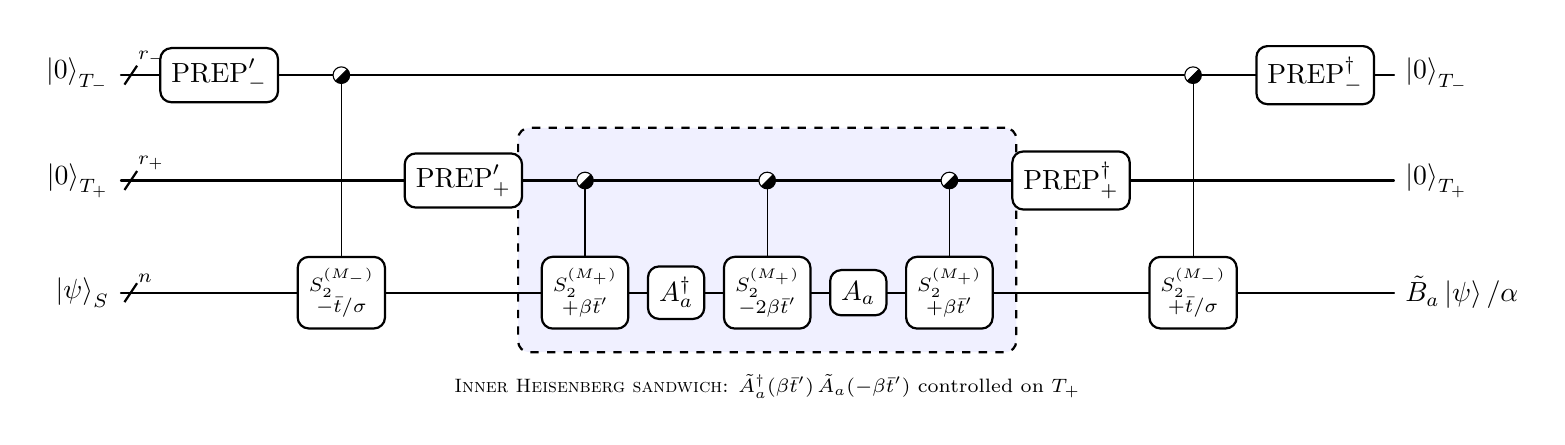
\begin{tikzpicture}
  \node[scale=1.0]{%
  \begin{quantikz}[row sep=0.6cm, column sep=0.25cm]
  %
  % Cell-by-cell layout (14 cells per row):
  %   1: \lstick                  (left label)
  %   2: wire decl                (\qwbundle{...})
  %   3: PREP'_-  (signed, outer)
  %   4: Ctrl-Trott outer^-       (S_2(-bar t / sigma) on S, ctrl on T_-)
  %   5: PREP'_+  (signed/phased, inner)
  %   6: Ctrl-Trott inner^+       (S_2(+beta bar t') on S, ctrl on T_+)
  %   7: A_a^dag on S             (inner Heisenberg sandwich, left)
  %   8: Ctrl-Trott inner^-2      (S_2(-2 beta bar t') on S, ctrl on T_+)
  %   9: A_a on S                 (inner Heisenberg sandwich, right)
  %  10: Ctrl-Trott inner^+       (S_2(+beta bar t') on S, ctrl on T_+)
  %  11: PREP_+^dag  (magnitude, inner UNPREP)
  %  12: Ctrl-Trott outer^+       (S_2(+bar t / sigma) on S, ctrl on T_-)
  %  13: PREP_-^dag  (magnitude, outer UNPREP)
  %  14: rstick
  %
  % ==================================================================
  % Row 1:  T_-  (outer time register; controls cells 4 and 12)
  % ==================================================================
    \lstick{$\ket{0}_{T_-}$}
      & \qwbundle{r_-}
      & \gate{\text{PREP}'_-}
      & \ctrl[style=halfctrl]{2}
      & \qw
      & \qw
      & \qw
      & \qw
      & \qw
      & \qw
      & \qw
      & \ctrl[style=halfctrl]{2}
      & \gate{\text{PREP}_-^\dagger}
      & \rstick{$\ket{0}_{T_-}$}\qw
      \\
  %
  % ==================================================================
  % Row 2:  T_+  (inner time register; controls cells 6, 8, 10;
  %              prepared in cell 5, uncomputed in cell 11)
  % ==================================================================
    \lstick{$\ket{0}_{T_+}$}
      & \qwbundle{r_+}
      & \qw
      & \qw
      & \gate{\text{PREP}'_+}
      & \ctrl[style=halfctrl]{1}
      \gategroup[2,steps=5,style={dashed,rounded corners,fill=blue!6,inner sep=5pt},
                 background,label style={label position=below,yshift=-0.35cm,anchor=north}]
        {\scriptsize \textsc{Inner Heisenberg sandwich}:
         $\tilde{A}_a^\dagger(\beta\bar t')\,\tilde{A}_a(-\beta\bar t')$
         controlled on $T_+$}
      & \qw
      & \ctrl[style=halfctrl]{1}
      & \qw
      & \ctrl[style=halfctrl]{1}
      & \gate{\text{PREP}_+^\dagger}
      & \qw
      & \qw
      & \rstick{$\ket{0}_{T_+}$}\qw
      \\
  %
  % ==================================================================
  % Row 3:  S  (system register; target of every controlled evolution
  %             and of the two jump applications A_a^dag, A_a)
  % ==================================================================
    \lstick{$\ket{\psi}_S$}
      & \qwbundle{n}
      & \qw
      & \gate{\substack{S_2^{(M_-)} \\[-1pt] \scriptstyle -\bar t/\sigma}}
      & \qw
      & \gate{\substack{S_2^{(M_+)} \\[-1pt] \scriptstyle +\beta\bar t'}}
      & \gate{A_a^\dagger}
      & \gate{\substack{S_2^{(M_+)} \\[-1pt] \scriptstyle -2\beta\bar t'}}
      & \gate{A_a}
      & \gate{\substack{S_2^{(M_+)} \\[-1pt] \scriptstyle +\beta\bar t'}}
      & \qw
      & \gate{\substack{S_2^{(M_-)} \\[-1pt] \scriptstyle +\bar t/\sigma}}
      & \qw
      & \rstick{$\tilde B_a\ket{\psi}/\alpha$}\qw
  \end{quantikz}%
  };
  \end{tikzpicture}%
  }
  \caption{Nested-LCU block encoding $U_{B_a}$ of the Trotterized coherent
  Metropolis term $\tilde{B}_a/\alpha$ with $\alpha=\lVert b_-\rVert_1\lVert b_+\rVert_1$
  (Alg.~\ref*{alg:coh}, \eqref{eq:B-block-encoding}), on outer/inner time
  registers $T_\mp$; projection on $\ket{0}_{T_-}\!\ket{0}_{T_+}$ is implicit.
  Half-filled controls denote uniform (SELECT) control over the bundled time
  registers. Following \cite[Fig.~4]{chen2023efficient},
  $\text{PREP}'_\pm$ prepares the signed/phased state
  $\sum_{\bar t}[b_\pm(\bar t)/\sqrt{|b_\pm(\bar t)|}]\ket{\bar t}/\sqrt{\lVert b_\pm\rVert_1}$
  and $\text{PREP}_\pm$ the magnitude state
  $\sum_{\bar t}\sqrt{|b_\pm(\bar t)|/\lVert b_\pm\rVert_1}\ket{\bar t}$,
  so that amplitudes multiply to the signed kernel $b_\pm(\bar t)$. Controlled
  evolutions are Trotterized with the second-order Strang splitting $S_2^{(M_\pm)}$.}
  \label{fig:block-encoding-ba-halfctrl}
\end{figure}

\end{document}
 in the main thesis,
%        or compile standalone.
%
% Differences from block-encoding-ba.tex:
%   (1) \ctrl{n}  -->  \ctrl[style=halfctrl]{n}  on every SELECT control
%       (cells 4, 12 on T_-; cells 6, 8, 10 on T_+).
%   (2) Signed/complex LCU fix, matching Chen et al. Fig. 4:
%         - left-side PREP on each register prepares the *signed* state
%               |b'_->   = sum_t   [b_-(t)/sqrt(|b_-(t)|)] / sqrt(||b_-||_1) |t>
%               |b'_+>   = sum_t'  [b_+(t')/sqrt(|b_+(t')|)] / sqrt(||b_+||_1) |t'>
%           denoted PREP'_- and PREP'_+ (primed).
%         - right-side PREP on each register prepares the *magnitude* state
%               |b_->    = sum_t   sqrt(|b_-(t)| / ||b_-||_1) |t>
%               |b_+>    = sum_t'  sqrt(|b_+(t')| / ||b_+||_1) |t'>
%           denoted PREP_- and PREP_+ (unprimed), and enters the circuit as
%           its adjoint PREP^dag on the right end.
%       With these two distinct preps, the left*right amplitude product on
%       each register is
%               [sgn/phase(b_-) sqrt(|b_-|)] * sqrt(|b_-|)  =  b_-
%       recovering the correctly signed/phased linear combination.
%       A symmetric PREP/PREP^dag on both ends would instead block-encode
%       |b_-(t)| (losing the sign), which is the wrong operator.
%
\documentclass{article}
\usepackage[margin=1cm]{geometry}
\usepackage{tikz}
\usetikzlibrary{quantikz2}
\usepackage{amsmath,amssymb}
\usepackage{braket}

\newcommand{\ee}{\mathrm{e}}
\newcommand{\ii}{\mathrm{i}}

% Rounded corners on all gates globally
\tikzset{operator/.append style={rounded corners}}

% Half-filled control: disk split by a / diagonal,
% lower-right triangle black, upper-left triangle white.
% Denotes a SELECT-style control that is *uniform* over a bundled register,
% as opposed to a computational-basis control on a single wire.
\tikzset{
  halfctrl/.style={
    circle, draw=black, line width=0.4pt,
    fill=white, minimum size=6pt, inner sep=0pt,
    path picture={
      \fill[black]
        (path picture bounding box.south west) --
        (path picture bounding box.south east) --
        (path picture bounding box.north east) -- cycle;
      \draw[black, line width=0.3pt]
        (path picture bounding box.south west) --
        (path picture bounding box.north east);
    }
  }
}

\begin{document}
\pagestyle{empty}

\begin{figure}[ht]
  \centering
  \makebox[\textwidth][c]{%
  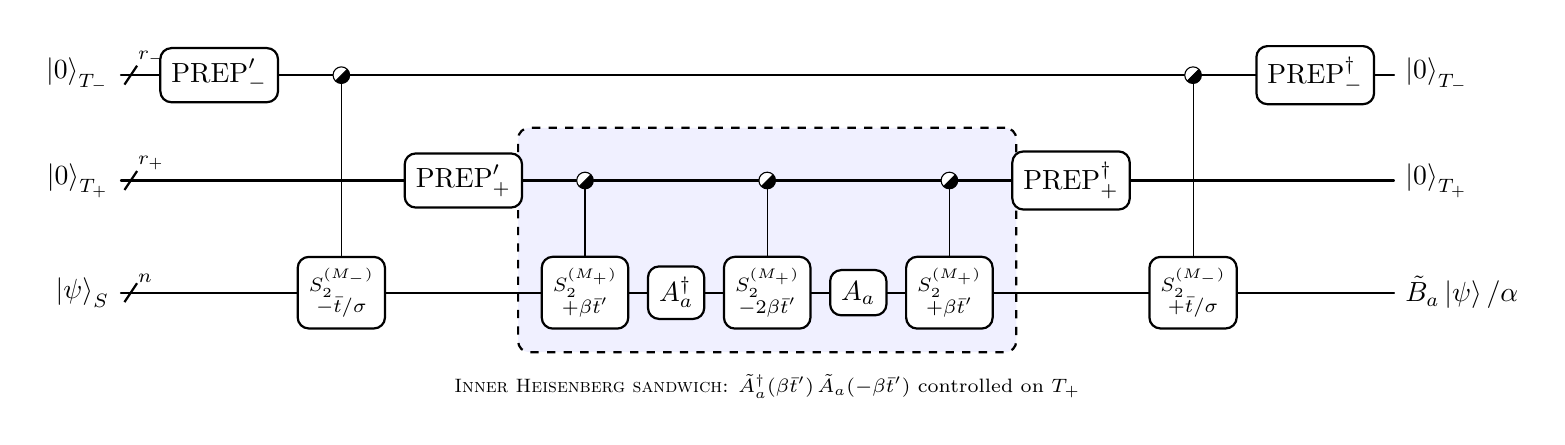
\begin{tikzpicture}
  \node[scale=1.0]{%
  \begin{quantikz}[row sep=0.6cm, column sep=0.25cm]
  %
  % Cell-by-cell layout (14 cells per row):
  %   1: \lstick                  (left label)
  %   2: wire decl                (\qwbundle{...})
  %   3: PREP'_-  (signed, outer)
  %   4: Ctrl-Trott outer^-       (S_2(-bar t / sigma) on S, ctrl on T_-)
  %   5: PREP'_+  (signed/phased, inner)
  %   6: Ctrl-Trott inner^+       (S_2(+beta bar t') on S, ctrl on T_+)
  %   7: A_a^dag on S             (inner Heisenberg sandwich, left)
  %   8: Ctrl-Trott inner^-2      (S_2(-2 beta bar t') on S, ctrl on T_+)
  %   9: A_a on S                 (inner Heisenberg sandwich, right)
  %  10: Ctrl-Trott inner^+       (S_2(+beta bar t') on S, ctrl on T_+)
  %  11: PREP_+^dag  (magnitude, inner UNPREP)
  %  12: Ctrl-Trott outer^+       (S_2(+bar t / sigma) on S, ctrl on T_-)
  %  13: PREP_-^dag  (magnitude, outer UNPREP)
  %  14: rstick
  %
  % ==================================================================
  % Row 1:  T_-  (outer time register; controls cells 4 and 12)
  % ==================================================================
    \lstick{$\ket{0}_{T_-}$}
      & \qwbundle{r_-}
      & \gate{\text{PREP}'_-}
      & \ctrl[style=halfctrl]{2}
      & \qw
      & \qw
      & \qw
      & \qw
      & \qw
      & \qw
      & \qw
      & \ctrl[style=halfctrl]{2}
      & \gate{\text{PREP}_-^\dagger}
      & \rstick{$\ket{0}_{T_-}$}\qw
      \\
  %
  % ==================================================================
  % Row 2:  T_+  (inner time register; controls cells 6, 8, 10;
  %              prepared in cell 5, uncomputed in cell 11)
  % ==================================================================
    \lstick{$\ket{0}_{T_+}$}
      & \qwbundle{r_+}
      & \qw
      & \qw
      & \gate{\text{PREP}'_+}
      & \ctrl[style=halfctrl]{1}
      \gategroup[2,steps=5,style={dashed,rounded corners,fill=blue!6,inner sep=5pt},
                 background,label style={label position=below,yshift=-0.35cm,anchor=north}]
        {\scriptsize \textsc{Inner Heisenberg sandwich}:
         $\tilde{A}_a^\dagger(\beta\bar t')\,\tilde{A}_a(-\beta\bar t')$
         controlled on $T_+$}
      & \qw
      & \ctrl[style=halfctrl]{1}
      & \qw
      & \ctrl[style=halfctrl]{1}
      & \gate{\text{PREP}_+^\dagger}
      & \qw
      & \qw
      & \rstick{$\ket{0}_{T_+}$}\qw
      \\
  %
  % ==================================================================
  % Row 3:  S  (system register; target of every controlled evolution
  %             and of the two jump applications A_a^dag, A_a)
  % ==================================================================
    \lstick{$\ket{\psi}_S$}
      & \qwbundle{n}
      & \qw
      & \gate{\substack{S_2^{(M_-)} \\[-1pt] \scriptstyle -\bar t/\sigma}}
      & \qw
      & \gate{\substack{S_2^{(M_+)} \\[-1pt] \scriptstyle +\beta\bar t'}}
      & \gate{A_a^\dagger}
      & \gate{\substack{S_2^{(M_+)} \\[-1pt] \scriptstyle -2\beta\bar t'}}
      & \gate{A_a}
      & \gate{\substack{S_2^{(M_+)} \\[-1pt] \scriptstyle +\beta\bar t'}}
      & \qw
      & \gate{\substack{S_2^{(M_-)} \\[-1pt] \scriptstyle +\bar t/\sigma}}
      & \qw
      & \rstick{$\tilde B_a\ket{\psi}/\alpha$}\qw
  \end{quantikz}%
  };
  \end{tikzpicture}%
  }
  \caption{Nested-LCU block encoding $U_{B_a}$ of the Trotterized coherent
  Metropolis term $\tilde{B}_a/\alpha$ with $\alpha=\lVert b_-\rVert_1\lVert b_+\rVert_1$
  (Alg.~\ref*{alg:coh}, \eqref{eq:B-block-encoding}), on outer/inner time
  registers $T_\mp$; projection on $\ket{0}_{T_-}\!\ket{0}_{T_+}$ is implicit.
  Half-filled controls denote uniform (SELECT) control over the bundled time
  registers. Following \cite[Fig.~4]{chen2023efficient},
  $\text{PREP}'_\pm$ prepares the signed/phased state
  $\sum_{\bar t}[b_\pm(\bar t)/\sqrt{|b_\pm(\bar t)|}]\ket{\bar t}/\sqrt{\lVert b_\pm\rVert_1}$
  and $\text{PREP}_\pm$ the magnitude state
  $\sum_{\bar t}\sqrt{|b_\pm(\bar t)|/\lVert b_\pm\rVert_1}\ket{\bar t}$,
  so that amplitudes multiply to the signed kernel $b_\pm(\bar t)$. Controlled
  evolutions are Trotterized with the second-order Strang splitting $S_2^{(M_\pm)}$.}
  \label{fig:block-encoding-ba-halfctrl}
\end{figure}

\end{document}
